\documentclass[a4paper,10pt]{article}
\usepackage[a4paper, total={7in, 8in}]{geometry}
\setlength\parindent{0pt}
\usepackage[utf8]{inputenc}
\usepackage{graphicx} 
\usepackage{amsmath}
\usepackage{amsfonts}
\usepackage{amssymb}
\usepackage{listings}
\usepackage{ragged2e}
\usepackage{listings}
\usepackage{color}
\setlength{\parskip}{\baselineskip}%
\setlength{\parindent}{0pt}%
\begin{document}

\begin{titlepage}
	\centering
	
\includegraphics[width=.6\textwidth]{liu-logo.png}\par
	\vfill
	{\scshape\Large TDDC17 ARTIFICIAL INTELLIGENCE\par}
	{\huge\bfseries Lab 6: Deep Learning\par}
	\vspace{1cm}
	{\large\itshape Robin Andersson (roban591) \\ Lawrence Thanakumar Rajappa (lawra776)\par}
	\vfill
	{\large \today\par}
\end{titlepage}

\definecolor{dkgreen}{rgb}{0,0.6,0}
\definecolor{gray}{rgb}{0.5,0.5,0.5}
\definecolor{mauve}{rgb}{0.58,0,0.82}

\lstset{frame=tb,
  language=Python,
  aboveskip=3mm,
  belowskip=3mm,
  showstringspaces=false,
  columns=flexible,
  basicstyle={\small\ttfamily},
  numbers=none,
  numberstyle=\tiny\color{gray},
  keywordstyle=\color{blue},
  commentstyle=\color{dkgreen},
  stringstyle=\color{mauve},
  breaklines=true,
  breakatwhitespace=true,
  tabsize=3
}

\section*{Part 2}
\textbf{Q1. In the gradient descent learning code below, please complete the gradient computation by inputing the
correct variables where there are question marks.We are using Tensorflow to automatically compute the gradient with
GradientTape (tape) similar to how you were taught above, but to do supervised learning which tensorflow node do
we compute the gradient of, and with regard to which variable? Please fill this in below.}

\begin{lstlisting}
tf.print("Loss before training:", training_loss(parameters))

for i in range(10):  # Adjust number of iterations as desired
  # Compute loss and optimize parameters using gradient descent
  with tf.GradientTape() as tape:  # Records tensor operations so it can be used for later derivation (gradients)
    loss = training_loss(parameters)  # Defines tensorflow node 'loss' as a function of...
  gradient = tape.gradient(loss, parameters) # Answer to Q1.
  tf.assign(parameters, parameters - 0.01 * gradient)   

tf.print("Loss after training:", training_loss(parameters))
tf.print("Parameters of linear model after training (intercept, slope):", parameters)

# Plotting
test_x = range(6) # Test inputs for x=0..6
test_y = model(test_x, parameters)  # Ask trained model for predictions
# Plot (NOTE: line comes from linear model assumption)
import matplotlib.pyplot as plt
_ = plt.plot(examples_x, examples_y, 'o', test_x, test_y, 'o-')
_ = plt.ylim([0,50])

\end{lstlisting}

\section*{Part 3}

\textbf{Q2. Show the math for why the first Dense layer has 100 480 parameters with these inputs and number of neurons}

The input for the first layer is (28,28) and number of neurons in the dense(hidden) layer is 128 neurons,
Number of biases for hidden layer is 128 neurons, hence
\begin{center}
	\begin{tabular}{l}
		$A$ = Number of inputs \\
		$B$ = Number of Neurons in the hidden layer \\
		$C$ = Number of biases for hidden layer \\
	\end{tabular}
\end{center}
\begin{equation*}
	(A * B) + C = (28*28*128)+128 = 100~480~\text{Parameters}
\end{equation*}


\textbf{Q3. Here you will evaluate different mini-bach sizes for stochastic gradient descent (see the deep learning lecture). 
Please separately run the training code above with batch sizes of 1, 10, 100, 1000 and 60000. 
Write down the training times (you can use the first number in seconds, not the per sample time) and 
the training set accuracy reached, both in the first line of the output. 
This can randomly vary a bit between runs but it should give you an idea. 
In your lab report, plot both curves and reason about which batch size produced the most accuracy 
given the time spent, i.e. which batch size would be best to start the training with?}

Please find the table below with batch size, duration and accuracy,
\begin{center}
	\setlength{\arrayrulewidth}{1.0pt}
	\begin{tabular}{|c|c|c|c|}
		\hline
		 \textbf{Batch Size} & \textbf{Time Duration in (seconds)} & \textbf{Accuracy \%}\\ [1.5ex]
		\hline
		1 & 109 &81.23\\
		\hline
		10 & 15 &82.56\\
		\hline
		100 & 3 &81.78\\
		\hline
		1000 & 2 &72.81\\
		\hline
		60000 & 2 &6.16\\
		\hline
	\end{tabular}
\end{center} 
\begin{center}
	\setlength{\arrayrulewidth}{1.0pt}
	\begin{tabular}{|c|c|}
		\hline
		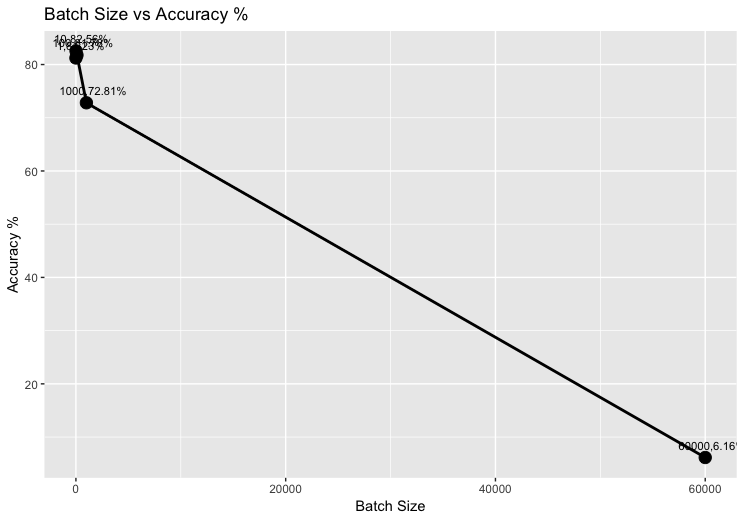
\includegraphics[width=.5\textwidth]{Batch_Size_Accuracy.png}\\
		\hline
		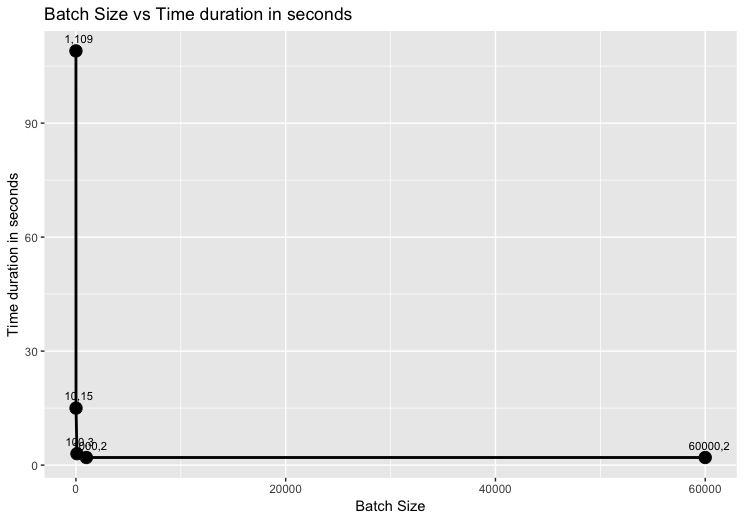
\includegraphics[width=.5\textwidth]{Batch_Size_Time.png}\\
		\hline
	\end{tabular}
\end{center}

It is better to use batch size of 10 which has good accuracy than other batch sizes as well as execution time is minimal.
Moreover,batch size has an important role in optimization technique because parallelization of stochastic gradient descent
in deep learning is limited, if we use small batch size. In order to solve this, we are using large batch size. When using
batch size of 10, the usage of memory is less during training and also networks train faster using mini batches because
we update weights after each propagation. But sometime you could ask, why not use a batch size of 1? Using this batch size and calculating
gradient descent for the entire dataset takes lot of memory to process and gradient trajectory lands in the bad spot i.e. saddle point.
Hence, considering the above points, it is better to use 10 as the batch size with respect to this dataset.

\end{document}